\documentclass[serif,10pt]{beamer}
%%%%%%%%%%%%%%%%%%%%%%%%%%%%%%%%%%%%%%%%%%%%%%%%%%%%%%%%%%%%%%%%%%%%%%%%%%%%%%%%%%%%%%%%%%%%%%%%%%%%%%

\mode<presentation> {
  \usetheme{Madison}
%    \usetheme[left,hideallsubsections,width=1cm]{UWThemeB}
  \usefonttheme[onlymath]{serif}

}

% % % % to make navigation two lines
\usepackage{ragged2e}

\makeatletter
\setbeamertemplate{section in head/foot}{%
    \parbox[c][0.33cm][t]{\dimexpr(\textwidth-1.3cm)/\beamer@sectionmax\relax}{%
        \RaggedRight\fontsize{4}{4}\selectfont\insertsectionhead}}
\setbeamertemplate{footline}[frame number]
\makeatother
% % % %

\usepackage{alltt}
\usepackage{tikz}                   % For TikZ graphicss
\usepgflibrary{patterns}            % This is to get "dots" and stuff in the graphics
\usepgflibrary{snakes}              % This is to get the "snakes" in the LD picture
\usepackage{hyperref}
\usepackage[english]{babel}
\usepackage[latin1]{inputenc}
\usepackage{mathptmx}               % Hace lucir la matematica rara
\usepackage{helvet}
\usepackage{courier}

\usepackage[absolute,overlay]{textpos}
\usepackage{graphicx}
\usepackage{multirow}
\usepackage{scalefnt}
\usepackage[T1]{fontenc}            % Note that the encoding and the font should match. If T1
                                    % does not look nice, try deleting the line with the fontenc.
\usepackage{colortbl}
\usepackage{color}
\definecolor{light-gray}{gray}{0.75}
\def\textcol{blue}

\setlength\fboxsep{3pt}
\setlength\fboxrule{1pt}

\setbeamertemplate{blocks}[rounded][shadow=true]
\setbeamertemplate{navigation symbols}{}

%Personal definitions - Bayes Regression
\def\bsb{\boldsymbol \beta}
\def\bsa{\boldsymbol \alpha}
\def\bsm{\boldsymbol \mu}
\def\bsS{\boldsymbol \Sigma}
\def\bsx{\boldsymbol \xi}

\title[Introduction]{Introduction to Loss Data Analytics}

\date[Fall 2017]{Fall 2017}

\begin{document}

\frame{\titlepage}

\begin{frame}
  \frametitle{Outline}
    %\tableofcontents[part=1,pausesections]
     \tableofcontents[part=1]
\end{frame}

\part<presentation>{Main Talk}


\section[Relevance]{Relevance of Analytics}

\begin{frame}
\frametitle{Relevance of Insurance} By almost any measure, insurance
is a major economy activity \vspace{2mm}

  \begin{itemize}
\item On a global level, insurance premiums comprised about 6.3\% of the world gross domestic product (GDP) in 2013 (Source: International Insurance Fact Book:
2015) \vspace{2mm}
  \begin{itemize}
\item  Premiums accounted for 11.2\% of GDP in Japan \vspace{2mm}
\item  Represented 7.5\% of GDP in the United States \vspace{2mm}
\end{itemize} \vspace{4mm}

\item On a personal level: \vspace{2mm}

  \begin{itemize}
\item Almost everyone owning a home has insurance to protect themselves in the event of a fire, hailstorm, or some other calamitous
event \vspace{2mm}
\item Almost every country requires insurance for those driving a
car \vspace{2mm}
\end{itemize}\end{itemize}
\end{frame}

\begin{frame}
\frametitle{Analytics and Loss Data}
 \begin{itemize}
\item  Insurance is big business \vspace{2mm}

 \item  Because of the size, it is not surprising that these firms employ analytics in the same manner as other large
 corporations \vspace{2mm}

  \item  These areas include (i) sales and marketing, (ii)  compensation analysis, (iii) productivity analysis, and (iv) financial forecasting. For example, in sales and
  marketing: \vspace{2mm}

 \begin{itemize}
 \item Predict customer behavior/needs (target appropriate
 customers) \vspace{2mm}
 \item Anticipate customer reactions to promotions/rate changes \vspace{2mm}
 \item Manage acquisition costs (online sales, agent compensation) \vspace{2mm}
\end{itemize}
\item One could introduce analytics from many perspectives; we focus on \textit{loss data}, also known as \textit{insurance claims} or \textit{insurance amounts}
\end{itemize}
\end{frame}

\begin{frame}
\frametitle{What is Analytics?}

 \begin{itemize}
 \item Insurance is a data-driven industry -- analytics is a key to deriving information from
 data \vspace{2mm}

  \item But what is analytics? \vspace{2mm}

  \pause

  \item Some alternative descriptors: \vspace{2mm}
   \begin{itemize}
 \item ``business intelligence'' may focus on processes of collecting data, often through databases and data
 warehouses \vspace{2mm}
 \item ``business analytics'' utilizes tools and methods for statistical analyses of
 data \vspace{2mm}
  \item ``data science'' can encompass broader applications in many scientific
  domains \vspace{2mm}
  \end{itemize}
  \pause
  \item \textcolor{red}{Analytics} -- the process of using data to make
  decisions \vspace{2mm}
     \begin{itemize}
  \item This process involves gathering data, understanding models of uncertainty, making general inferences, and communicating
  results \vspace{2mm}
    \end{itemize}
\end{itemize}\end{frame}


\begin{frame}
\frametitle{Insurance Processes}
  \begin{itemize}
\item How does data arise from an insurer?
\item In a ``micro'' oriented view, we can think specifically about what happens to a contract at various stages of its existence
\end{itemize}
\vspace{-.15in}
\begin{figure}[htp]
\begin{center}
    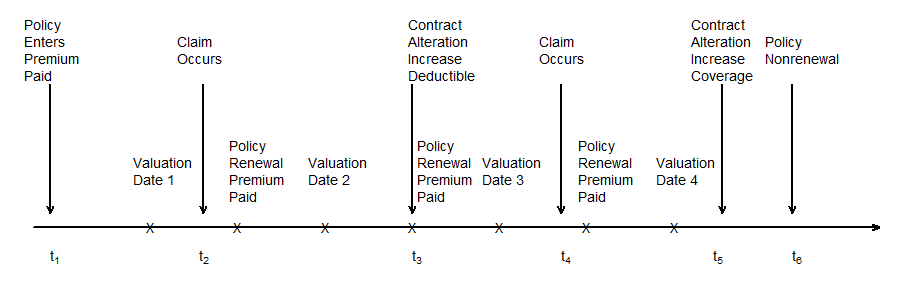
\includegraphics[scale = 0.5, bb = 400 220 100 100]{Figures/StochOperationsD.PNG}
    \caption{\label{F:StochOperations}\small Timeline of a Typical Insurance Policy. Arrows mark the occurrences of random events.}
\end{center}
\end{figure}
\end{frame}


\section{Variable Types}

\begin{frame}
\frametitle{Variable Types}
  \begin{itemize}
\item As in many areas of disciplined thought: \vspace{2mm}
  \begin{itemize}
\item Work with data (summarize) \vspace{2mm}
\item Represent data using models \vspace{2mm}
\item Use models calibrated with data to make decisions \vspace{2mm}
\end{itemize}
\item As a first step, it is helpful to classify a variable into one of several
types \vspace{2mm}
\item This classification drives the summarization and modeling decisions that we will
make
\end{itemize}
\end{frame}

\begin{frame}
\frametitle{Variable Types}
\begin{table}[htp]\scalefont{0.65}
  \begin{center}
\begin{tabular}{l|l} \hline
{\bf Variable Type} & {\bf Example} \\\hline
{\it Qualitative} &            \\
    Binary &        Sex \\
Categorical (Unordered, Nominal) & Territory (e.g., state/province) in which an insured resides \\
Ordered Category (Ordinal) & Claimant satisfaction (five point scale ranging from 1=dissatisfied \\
& ~~~ to 5 =satisfied) \\\hline
{\it Quantitative} &            \\
Continuous & Policyholder's age, weight, income \\
  Discrete & Amount of deductible \\
Count & Number of insurance claims \\
Combinations of  & Policy losses, mixture of 0's (for no loss)  \\
~~~ Discrete and Continuous & ~~~and positive claim amount \\
Interval Variable & Driver Age: 16-24 (young), 25-54 (intermediate),  \\
& ~~~55 and over (senior) \\
Circular Data & Time of day measures of customer arrival \\ \hline
{\it Multivariate Variable} &            \\
High Dimensional Data & Characteristics of a firm purchasing worker's compensation \\
& ~~~insurance (location of plants, industry, number of employees, \\
&~~~and so on) \\
Spatial Data & Longitude/latitude of the location an insurance hailstorm claim \\
Missing Data & Policyholder's age (continuous/interval) and ``-99'' for \\
&~~~ ``not reported,'' that is, missing \\
Censored and Truncated Data & Amount of insurance claims in excess of a deductible \\
Aggregate Claims & Losses recorded for each claim in a motor vehicle policy. \\
Stochastic Process Realizations & The time and amount of each occurrence of an insured loss \\ \hline
\end{tabular}\end{center}
\end{table}
\end{frame}

\section{Insurance Company Operations}

\begin{frame}%[shrink=20]
\frametitle{Insurance Company Operations I} \textit{Insurer's
Viewpoint:}
\newline\checkmark Need ways of bringing money in, paying it out, managing costs, and making sure that we have enough money to meet
obligations \vspace{2mm}
\newline\checkmark Insurers aggregate detailed insurance processes into larger ``operational''
units \vspace{2mm}
  \begin{itemize}
 \item Initiating Insurance \vspace{2mm}
\begin{itemize}
 \item Offer right price for the right risk (underwriting) \vspace{2mm}
 \item Avoid adverse selection \vspace{2mm}
 \end{itemize}
 \item Renewing Insurance \vspace{2mm}
   \begin{itemize}
 \item Retain profitable customers longer \vspace{2mm}
 \item Update prices using experience (bonus-malus, credibility) \vspace{2mm}
\end{itemize}
\end{itemize}
\end{frame}

\begin{frame}%[shrink=20]
\frametitle{Insurance Company Operations II}
 \begin{itemize}
 \item Claims and Product Management \vspace{2mm}
 \begin{itemize}
  \item Detect and manage claims fraud \vspace{2mm}
 \item Manage claims costs (triaging, processing, adjustment decisions) \vspace{2mm}
 \item Understand excess layers for reinsurance and retention \vspace{2mm}
\end{itemize}
\item Reserving \vspace{2mm}
 \begin{itemize}
 \item Predict future obligations: set an adequate reserve to fund losses that have been incurred but not developed \vspace{2mm}
\item Quantify the uncertainty of the estimates \vspace{2mm}
\item Match projections of obligations to income streams \vspace{2mm}
\item Consider ``lines of business;'' for non-life, typical lines
include personal auto, personal homeowners, commercial auto, etc.
\vspace{2mm}
\end{itemize}
\item Capital Allocation and Solvency \vspace{2mm}
 \begin{itemize}
\item Decide appropriate level of necessary capital \vspace{2mm}
\item Manage external stakeholders' expectations; regulators, rating agencies, reputation
\end{itemize}
\end{itemize}
\end{frame}

\begin{frame}[shrink=2]
\frametitle{Operations -- Initiating Insurance}
  \begin{itemize}
\item Setting the price of an insurance good can be a perplexing problem.
  \begin{itemize}
\item In manufacturing, the cost of a good is (relatively) known
\item In other areas of financial services, market prices are available
\item In many lines of insurance, start with an expected cost, add ``margins'' to account for the product's riskiness, expenses incurred in servicing the product, and a profit/surplus allowance for the insurance company.
\end{itemize} \pause
\item For some lines of business, especially automobile and homeowners insurance, analytics has served to sharpen the market by making the calculation of the good's expectation more precise.
\item Pricing strategies now routinely involve generalized linear model (GLM) techniques
\item \textit{Underwriting}, the process of classifying risks into homogenous categories and assigning policyholders to these categories, lies at the core of ratemaking.  \begin{itemize}
\item Policyholders within a class have similar risk profiles and so are charged the same insurance price.
\end{itemize}\end{itemize}
\end{frame}

\begin{frame}[shrink=2]
\frametitle{Big Data}
  \begin{itemize}
\item Traditionally, insurers use information reported by policyholders on application forms, combined with selected external sources.
   \begin{itemize}
\item  E.g., police reports for automobile insurance or medical exam results for life insurance.
\item Many variables are categorical, making even limited info complex.
\end{itemize}
\item Now, there is interest in collecting more information about policyholders
   \begin{itemize}
\item An early example was the use of credit scores by Progressive Insurance for automobile insurance.
\item Ethically permissible? - these debates are important.
\item From a statistician's viewpoint, these additional sources have proven to be significant from hypothesis testing, predictive, and economic viewpoints.
 \end{itemize}
 \pause
\item Policyholders are also agreeing to let insurers gather more data about them for risk classification purposes. \begin{itemize}
\item  The best example is the GPS and cameras that are mounting in cars for monitoring how much and how a policyholder drives.
\item There are many that feel that this will represent a tremendous benefit to society.% For example, if insurers can reliably monitor how much a person drives, then insurance can be priced on usage basis (like gas/petrol), inducing people to drive less. Estimates indicate that if this takes hold in the future, we will be able to provide substantial help to the environment.
\end{itemize}

\end{itemize}
\end{frame}



\begin{frame}
\frametitle{Operations -- Renewing Insurance}
  \begin{itemize}
\item Renewal analytics are similar to initial underwriting but a little different. In addition to (contract initiation) rating variables, we also have claims history.
      \begin{itemize}
\item Rating variables (e.g., credit score) may evolve over time
\item Common to use history (e.g., whether a claim has occurred in the last three years)
  \end{itemize}
  \item Ways to incorporate experience into prices
    \begin{itemize}
\item a ``bonus-malus'' system where prior claim frequency is used to prospectively adjust premiums. Bonus-malus methods of experience rating are used extensively in automobile insurance pricing in Europe and Asia,
\item ``credibility'' adjusted prices that are a blend of a manual rate with past experience - used since the 1920's
\item bonus-malus and credibility are prospective systems. In life insurance, ``dividends'' are awarded retrospectively.
    \end{itemize}
\end{itemize}
\end{frame}

\begin{frame}[shrink=2]
\frametitle{Operations -- Claims Management}
Insurance managers sometimes use the phrase ``\textit{claims leakage}'' to mean dollars lost through claims management inefficiencies.
\begin{itemize}
\item Fraud detection. Mitigating fraud is an important part of claims management process.
\item Management of claims severity
\begin{itemize}
\item Claims triaging. Just as in the medical world, early identification and appropriate handling of high cost claims (patients, in the medical world), can lead to dramatic company savings.
\item Claims processing. The goal is to use analytics to identify situations suitable for small claims handling processes and those for adjuster assignment to complex claims.
\item Adjustment decisions. Once a complex claim has been identified and assigned to an adjuster, analytic driven routines can be established to aid subsequent decision-making processes.
\end{itemize}
\item Expenses. Loss adjustment expenses are part of an insurer's cost of managing claims.
\begin{itemize}
\item Analytics can be used to reduce expenses directly related to claims handling (``allocated'') as well as general staff time for overseeing the claims processes (``unallocated'').
\item The insurance industry has high operating costs relative to other portions of the financial services sectors.
\end{itemize}
\end{itemize}
\end{frame}


\begin{frame}
\frametitle{Operations -- Claims and Product Management}
Analytics is used in:
  \begin{itemize}
\item Fraud
\item Claims Management
  \begin{itemize}
\item Fraud, Claims Triaging, Expense Allocation \end{itemize}
\item Product Management
  \begin{itemize}
\item Customer Loyalty, Price Optimization \end{itemize}
\item Portfolio Management
  \begin{itemize}
\item Portfolio risk distribution \end{itemize}
\item Reinsurance
\end{itemize}
\end{frame}


\begin{frame}
\frametitle{Operations -- Loss Reserving}
\begin{itemize}
\item The primary goal of loss reserving is to set an adequate reserve to fund losses that have been incurred but not yet developed.
\item Insurance companies are organized by ``lines of business''
\begin{itemize}
\item Top-level is life versus non-life
\item For non-life, typical lines include personal auto, personal homeowners, commercial auto, and so forth.
\end{itemize}
\item In non-life insurance, losses are arranged in a triangular fashion as they
develop over time and as different obligations are incurred from year to year.
\item This triangular format emphasizes the longitudinal and censored nature of the data.
\end{itemize}
\end{frame}

\begin{frame}
\frametitle{Loss Reserve Example}
\vspace{-.1in}
\begin{figure}[htp]
  \begin{center}
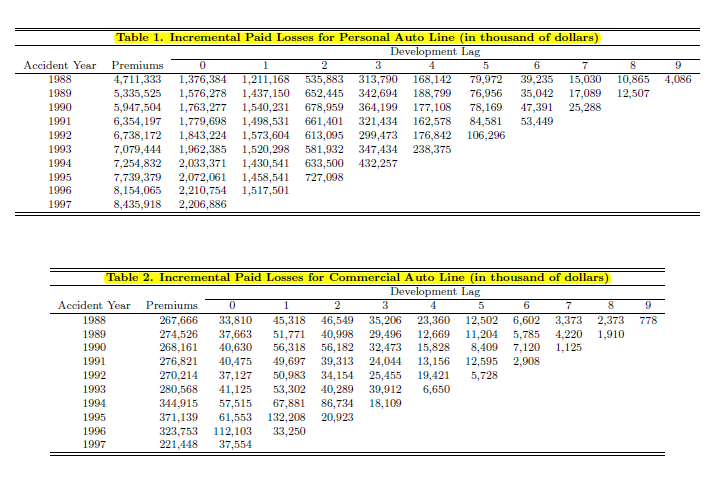
\includegraphics[width=1\textwidth]{Figures/LossFreesShi2011.png}
  \end{center}
\end{figure}
\vspace{-.1in}
Data from Frees and Shi (2011)
\end{frame}


\begin{frame}
\frametitle{Loss Reserve Example}
\vspace{-.1in}
\begin{figure}[htp]
  \begin{center}
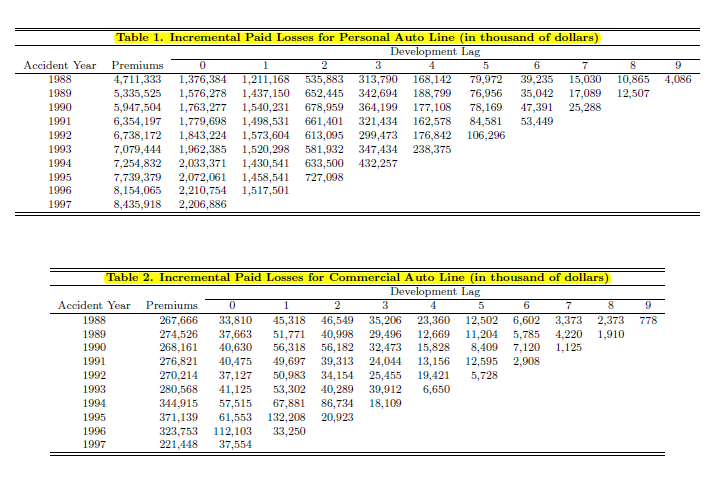
\includegraphics[width=2.2\textwidth]{Figures/LossFreesShi2011.png}
  \end{center}
\end{figure}
\end{frame}


\section[Case Study]{Case Study: Wisconsin Property Fund}

\begin{frame}
\frametitle{Wisconsin Property Fund}
  \begin{itemize}
\item The Wisconsin Office of the Insurance Commissioner administers the Local Government Property Insurance Fund
(LGPIF) \vspace{2mm}
\item Property coverage has been available since 1911 \vspace{2mm}
\item The fund insures property such as government buildings, schools, libraries, and motor
vehicles \vspace{2mm}
\item ``Local government''  entities include counties, cities, towns, villages, school districts, and library
boards \vspace{2mm}
  \begin{itemize} \item The fund has over 1,000 such entities \end{itemize}
\end{itemize}
%\hyperlink{AnalyticsOverview}{\beamergotobutton{Go to Analytics Overview}}
\end{frame}

\begin{frame}%[plain]
\frametitle{LGPIF Policyholder A}
\begin{figure}[htp]
  \begin{center}
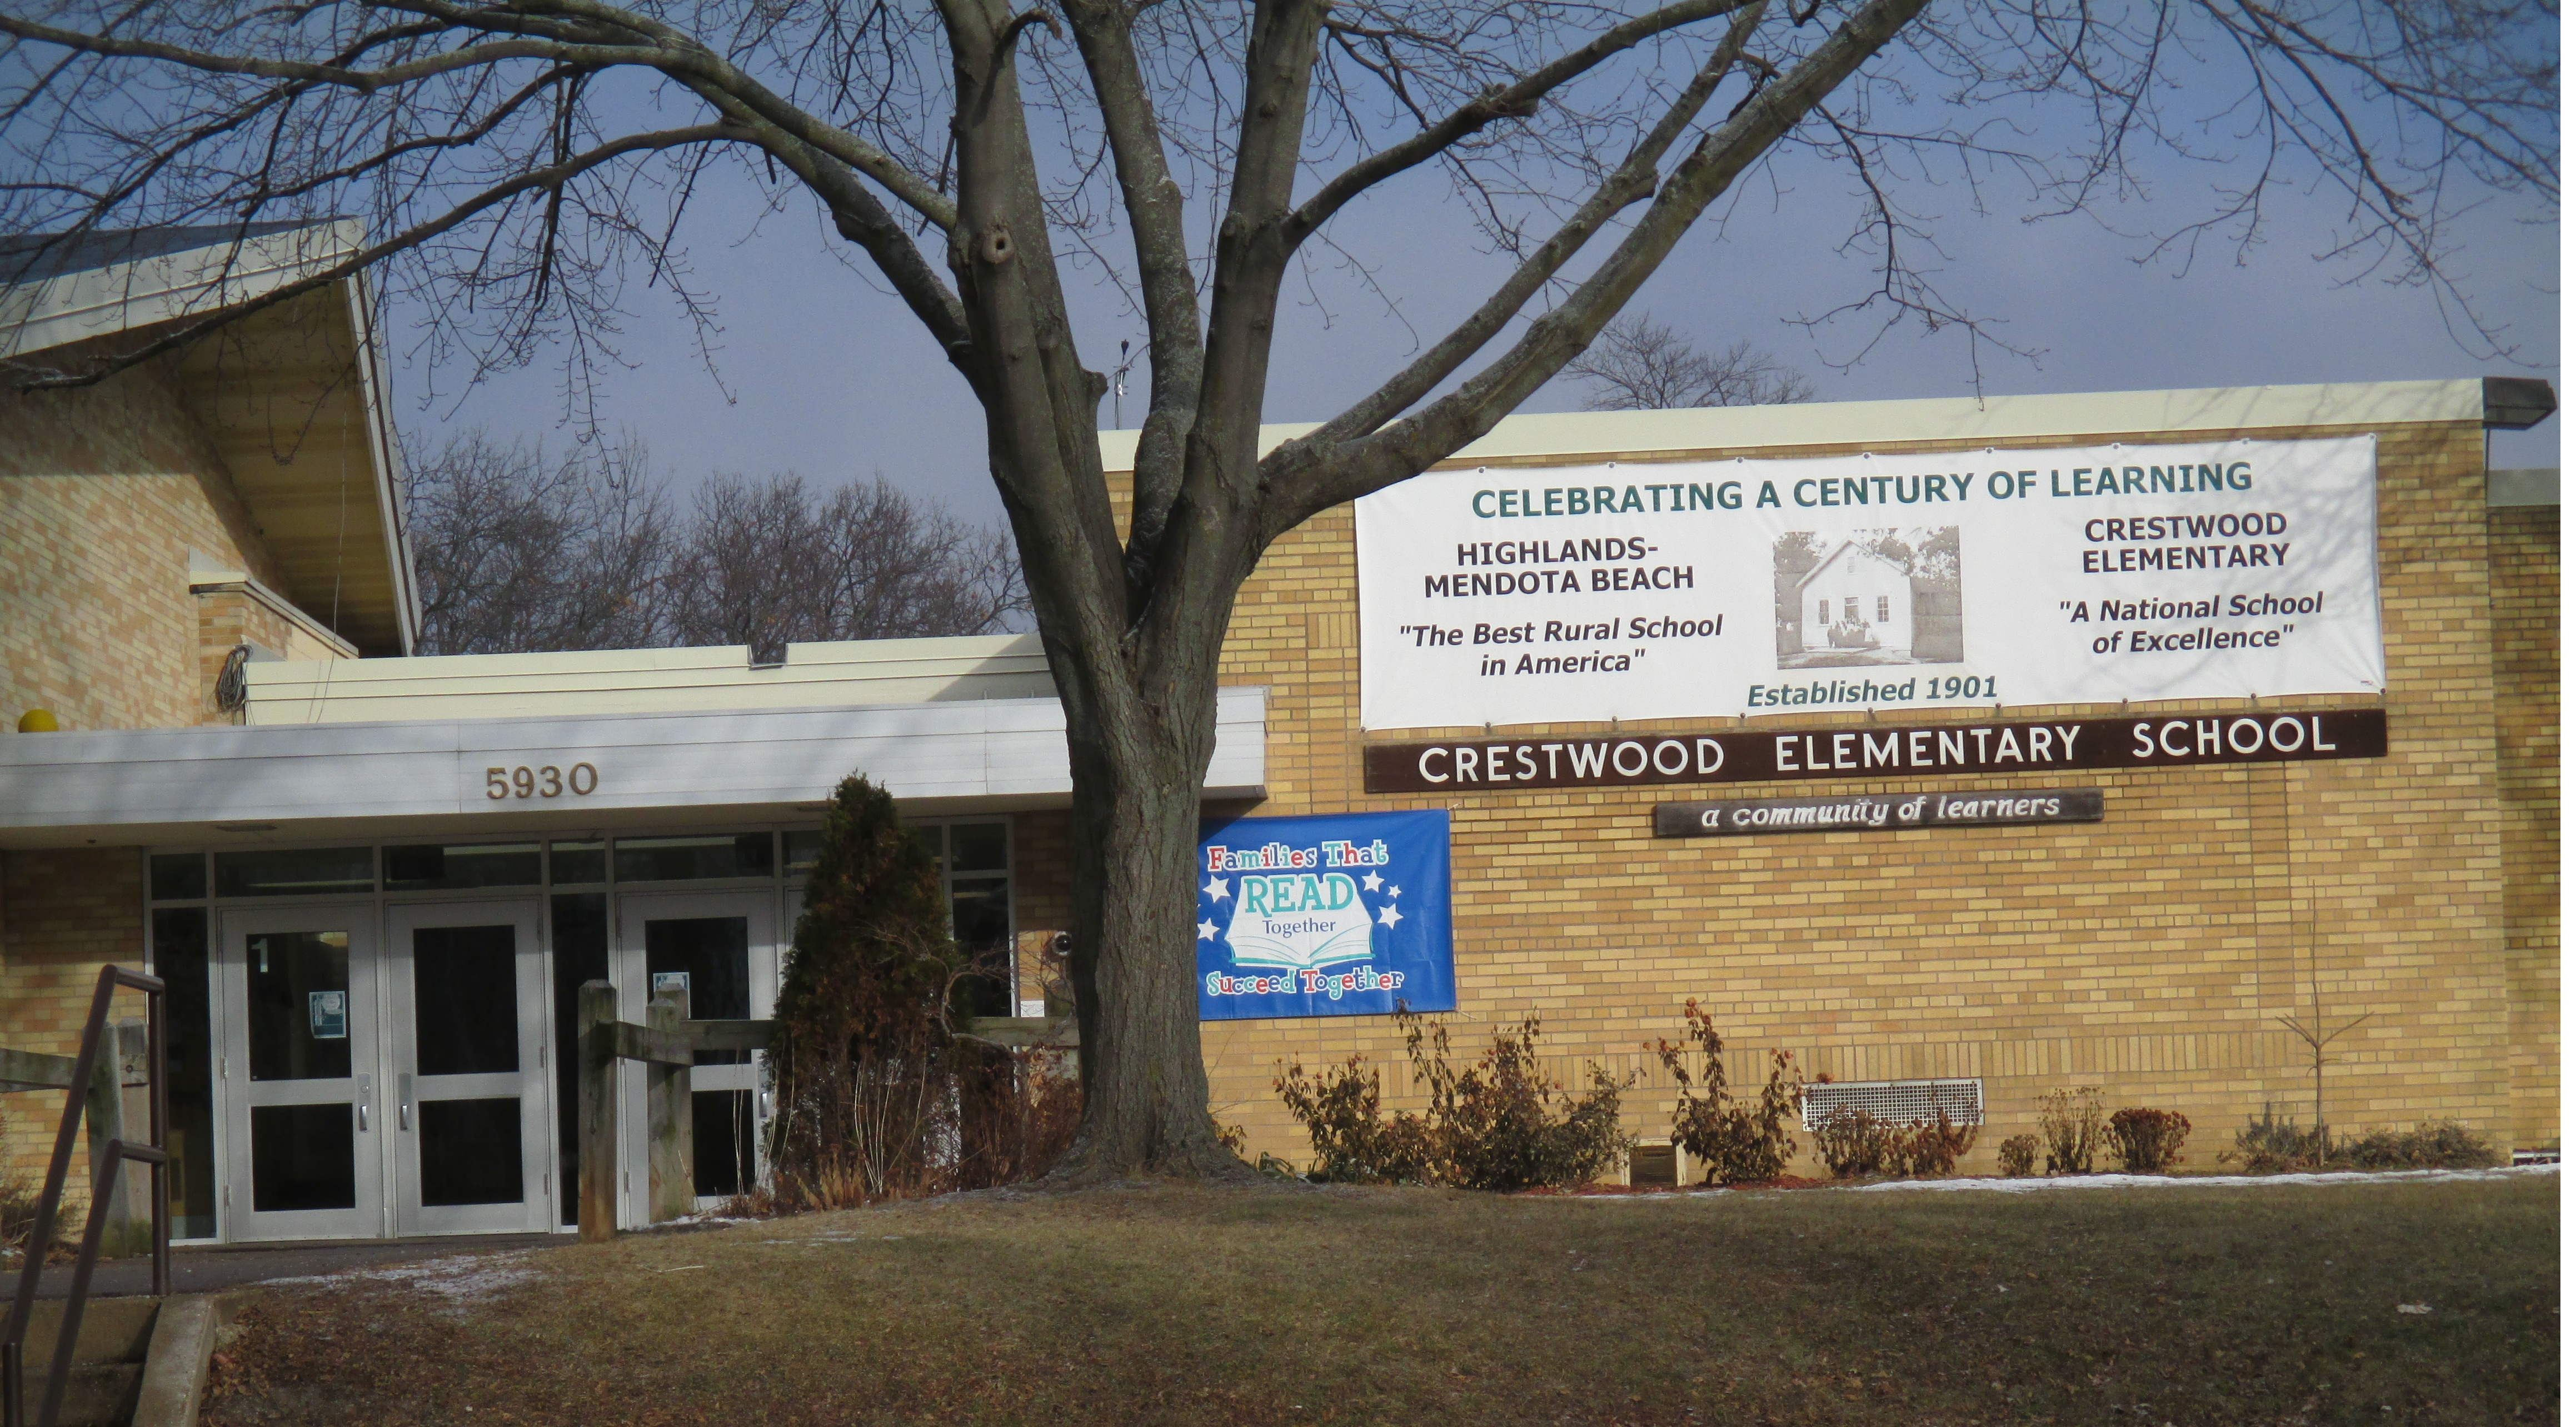
\includegraphics[scale = 0.075, bb = 300 300 300 300]{Figures/CrestwoodADec2014.JPG}
  \end{center}
\end{figure}

\vspace{0.2in}

  \begin{itemize}
\item Example --  Madison Metropolitan School District
  \begin{itemize}
\item it has 98 buildings, 18 major pieces of equipment (mowers, etc.), and 630 properties in the open (benches, playsets, goals,
etc.) \vspace{2mm}
\item the property coverage alone is \$640 million \vspace{2mm}
\item this is Crestwood Elementary School, one of the 98 buildings
\end{itemize}\end{itemize}
\end{frame}

\begin{frame}%[plain]
\frametitle{LGPIF Policyholder B}
\begin{figure}[t]
  \begin{center}
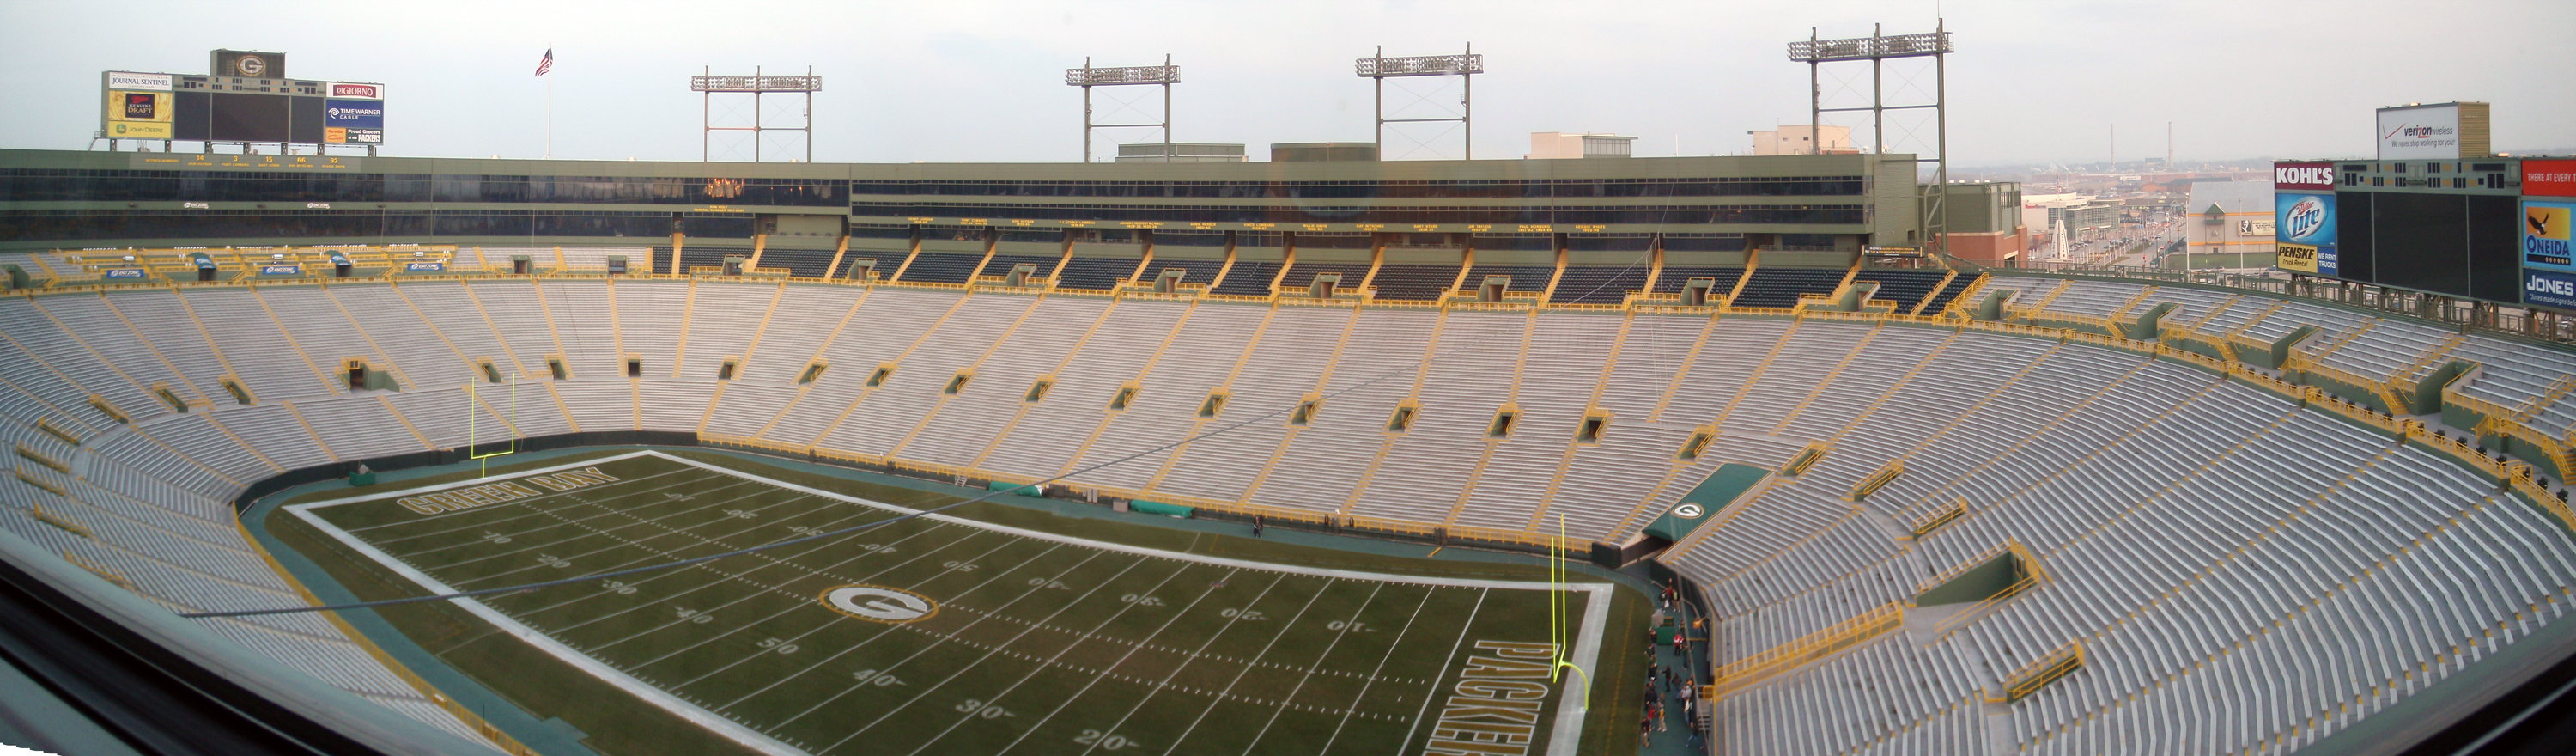
\includegraphics[scale = 0.25, bb = 300 300 600 300]{Figures/2009_pan_2_large.jpg}
  \end{center}
\end{figure}
  \begin{itemize}

  \vspace{1in}

\item The largest contract -- City of Green Bay \vspace{2mm}
  \begin{itemize}
\item contains 118 sites \vspace{2mm}
\item one of which is Lambeau Field  -- a stadium in which a professional football team, the Green Bay Packers,
plays \vspace{2mm}
\item Property coverage is approximately \$2.4 billion \vspace{2mm}
\item LGPIF has a separate terrorism reinsurance coverage for this property
\end{itemize}\end{itemize}
\end{frame}

\begin{frame}
\frametitle{Property Fund}
  \begin{itemize}
\item The fund receives approximately \$25 million in premiums each year and provides insurance coverage for about \$75
billion \vspace{2mm}
\item The fund offers three major groups of insurance coverage: building and contents, construction equipment, and motor
vehicles \vspace{2mm}
    \item For building and contents, the fund covers all property losses except those resulting from flood, earthquake, wear and tear, extremes in temperature, mold, war, nuclear reactions, and embezzlement or theft by an employee
\end{itemize}
\end{frame}

\subsection{Fund Claims Variables}

\begin{frame}
\frametitle{Claims Frequency (2010)}
  \begin{itemize}
\item The table shows 1,110 policyholders who have 1,377 claims \vspace{2mm}
\item Almost two-thirds (0.637) of the policyholders did not have any claims,  18.8\% had one claim and remaining  17.5\% (=1 - 0.637 - 0.188) had more than one
claim \vspace{2mm}
\item The policyholder with the highest number recorded 239 claims \vspace{2mm}
\item The average number of claims for this sample was 1.24 (=1377/1110)
\end{itemize}
\begin{table}[htbp]\scalefont{0.9}
  \centering
    \begin{tabular}{l | rrrr rrrr r r |r}
    \hline
Type &    \multicolumn{6}{c}{Number of Claims} &\\ \hline
Number&  0 &  1  & 2 &  3   &4  & 5   \\ \hline
Count & 707& 209  &86 & 40  &18 & 12   \\
Proportion & 0.637 &      0.188 &      0.077 &      0.036 &      0.016 &      0.011       \\\hline
\\ \hline
Number&  6  & 7  & 8  & 9 or more & Sum\\ \hline
Count & 9 &  4  & 6  & 19 &1,110\\
Proportion &  0.008 &      0.004 &      0.005 &      0.017 &      1.000 \\
    \hline
    \end{tabular}
 \end{table}

\end{frame}


\begin{frame}
\frametitle{Claims Severity (2010)}
  \begin{itemize}\scalefont{0.9}
\item 403 (=1110-707) policyholders had at least one claim \vspace{2mm}
\item The following summarizes the distribution of the average claims of those policyholders with
claims \vspace{2mm}
\begin{itemize}\item To illustrate, 209 policyholders had only one claim. Here, the claim amount equals the average
claim \vspace{2mm}
\end{itemize}\end{itemize}
\vspace{-.1in}
\begin{table}[htbp]\scalefont{0.9}
  \centering
    \begin{tabular}{rrrrrr}
    \hline
        &First &        &         &Third &\\
Minimum& Quartile    &Median &Mean     & Quartile     &Maximum \\  \hline
167    & 2,226        &4,951 & 56,330  &  11,900      & 12,920,000 \\
    \hline
    \end{tabular}
 \end{table}
\end{frame}

\begin{frame}
\frametitle{Claims Severity Distribution (2010)}
\begin{figure}[htp]
\begin{center}
    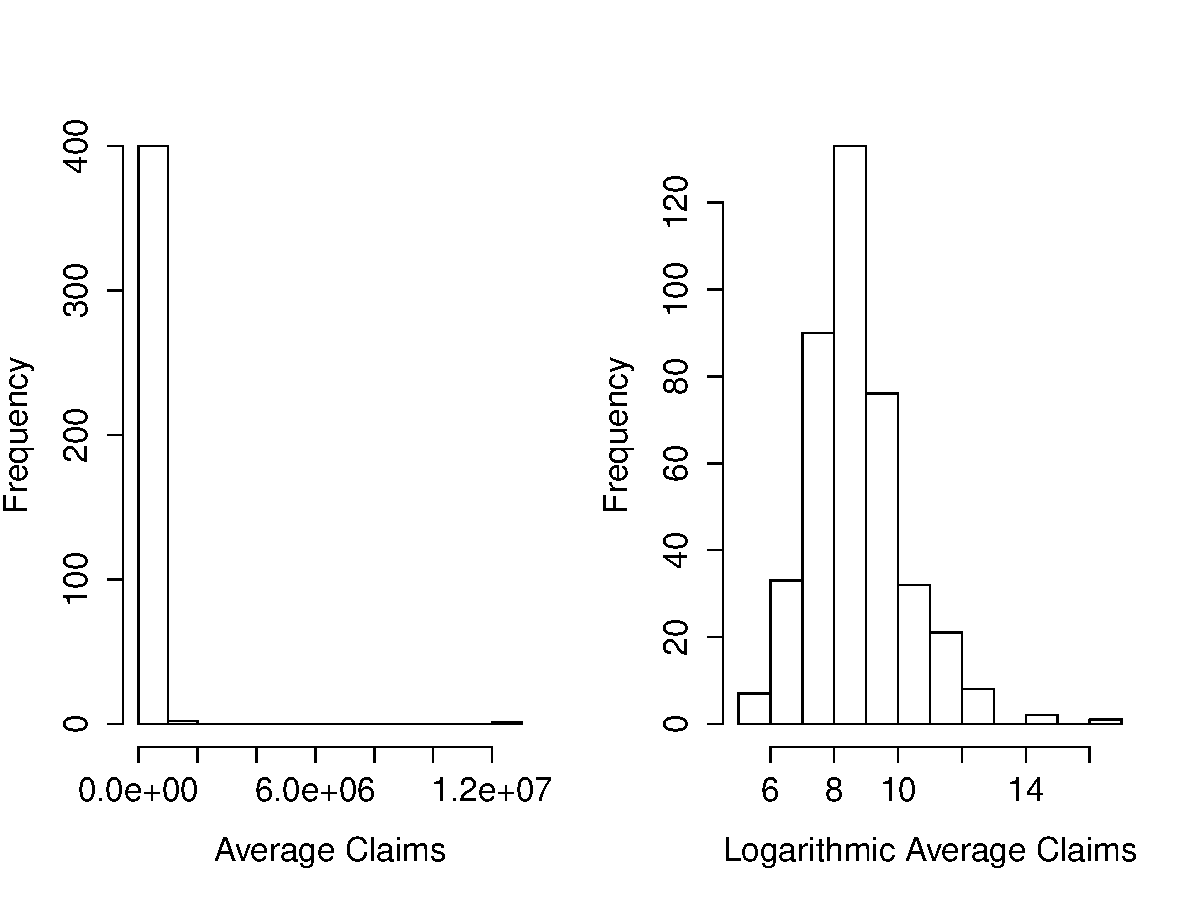
\includegraphics[scale = 0.4, bb = 400 220 100 100]{Figures/Severity1.pdf}
\end{center}
\end{figure}
\end{frame}


\begin{frame}
\frametitle{Claim Outcomes and Coverage by Year}
  \begin{itemize}
\item To increase the sample size, look to more years \vspace{2mm}
\item Average frequency is more stable than severity over years \vspace{2mm}
\item Coverage is stable and increasing \vspace{2mm}
\item Number of policyholders is stable but declining \vspace{2mm}
\end{itemize}
\begin{table}[htbp]\scalefont{0.9}
  \centering
    \begin{tabular}{l | rrrr}
    \hline
    \multirow{2}[4]{*}{Year} & Average & Average & Average & Number of \\
          & Frequency & Severity & Coverage & Policyholders \\
    \hline
      2006 &      0.951&     9,695 & 32,498,186 &       1,154 \\
      2007 &      1.167 &     6,544 & 35,275,949 &       1,138 \\
      2008 &      0.974 &     5,311 & 37,267,485 &       1,125 \\
      2009 &      1.219 &      4,572 & 40,355,382 &       1,112 \\
      2010 &      1.241 &     20,452 & 41,242,070 &       1,110 \\
    \hline
    \end{tabular}
  \label{T:CoverageBCIM}
\end{table}
\end{frame}

\begin{frame}
\frametitle{Claim Frequency and Severity, Deductibles, and Coverages}
  \begin{itemize}
\item The two outcomes variables are frequency and severity. Each has many zeros (more than
half) \vspace{2mm}
\item The two rating variables are deductible and coverages \vspace{2mm}
\item For each of the four distributions, Mean > Median, suggesting skewed
distributions \vspace{2mm}
\end{itemize}
\begin{table}[htp]
\begin{center}
\scalefont{0.9}
\begin{tabular}{l|rrrrrr} \hline
                 &   Minimum  &   Median   &   Mean &   Maximum \\ \hline
Claim Frequency  &          0 &          0 &   1.109 &        263      \\
Claim Severity   &          0 &          0 &   9,292 &   12,922,218  \\
Deductible       &        500 &      1,000 &   3,365 &   100,000 \\
Coverage (000's) &      8.937 &     11,354 &   37,281 &    2,444,797 \\
\hline
\end{tabular}
\end{center}
\end{table}
\end{frame}

\subsection{Fund Rating Variables}
\begin{frame}
\frametitle{Description of Rating Variables}
  \begin{itemize}
\item Identify variables types: binary, categorical, quantitative (discrete), and
continuous \vspace{2mm}
\end{itemize}
\begin{table}[htp]
\begin{center}
\scalefont{0.8}
\begin{tabular}{ l | l}
\hline
Variable    & Description \\
\hline
\multirow{2}{*}{{\tt EntityType}}   & Categorical variable that is one of six types:  (Village, City, \\
& ~~~ County, Misc, School, or Town) \\
\multirow{2}{*}{\tt LnCoverage} & Total building and content coverage, in logarithmic \\
 & ~~~ millions of dollars \\
\multirow{2}{*}{{\tt LnDeduct}}     & \multirow{2}{*}{Deductible, in logarithmic dollars} \\
\\
 \multirow{2}{*}{{\tt AlarmCredit}}  & Categorical variable that is one of four types:  (0\%, 5\%, 10\%, \\
 & ~~~ or 15\%),   for automatic smoke alarms in main rooms \\
\multirow{2}{*}{{\tt NoClaimCredit}}    & \multirow{2}{*}{Binary variable to indicate no claims in the past two years} \\
\\
\multirow{2}{*}{{\tt Fire5}}            & Binary variable to indicate the fire class is below 5 \\
& ~~~ (The range of fire class is $0\sim10$)\\
\hline
\end{tabular}
\scalefont{1.1111}
\end{center}
\end{table}
\end{frame}

\begin{frame}
\frametitle{Claims by Entity Type, Fire Class, and No Claim Credit}
  \begin{itemize}\scalefont{0.8}
\item There is substantial variation in the frequency and severity by entity
type \vspace{2mm}
\item As anticipated, lower frequency and severity when the policyholder had no claims in the past two years, ({\tt
NoClaimCredit=1}=1) \vspace{2mm}
\item Higher frequency and severity for the {\tt Fire5} (=1)
variable \vspace{2mm}
\begin{itemize}\scalefont{0.8}\item Counter-intuitive: one would expect lower claim amounts for those policyholders in areas with better public protection (when the protection code is five or less)
\end{itemize}\end{itemize}
\begin{table}[htp]
\begin{center}\scalefont{0.8}
\begin{tabular}{lrrr}
\hline
          &    Number of & Claim         & Average \\
Variable  &      Policies&      Frequency& Severity \\
\hline
 {\tt EntityType} \\
    Village               &            1,341  &            0.452  &              10,645  \\
    City                  &              793  &            1.941  &              16,924  \\
    County                &              328  &            4.899  &              15,453  \\
    Misc                  &              609  &            0.186  &              43,036  \\
    School                &            1,597  &            1.434  &              64,346  \\
    Town                  &              971  &            0.103  &              19,831  \\
    {\tt Fire5}=0         &            2,508  &            0.502  &              13,935  \\
    {\tt Fire5}=1         &            3,131  &            1.596  &              41,421  \\
    {\tt NoClaimCredit}=0 &            3,786  &            1.501  &              31,365  \\
    {\tt NoClaimCredit}=1 &            1,853  &            0.310  &              30,499  \\
    \hline
    Total                 &            5,639  &            1.109  &              31,206 \\
        \hline
    \end{tabular}
\scalefont{1.1111}\end{center}
\end{table}
\end{frame}


\begin{frame}
\frametitle{Claims Summary by Entity Type and Alarm Credit Category}
  \begin{itemize}\scalefont{0.8}
\item Counter-intuitive results for Alarm Credit. Would expect lower frequency/severity for 15\% alarm
credits \vspace{2mm}
\end{itemize}
\begin{table}[htbp]
  \centering
  \scalefont{0.66667}
    \begin{tabular}{l | rrr | rrr }
    \hline \hline
   & \multicolumn{3}{c|}{No Alarm Credit} & \multicolumn{3}{c}{Alarm Credit 5\%}  \\
    Entity & Claim & Avg.  & Num. & Claim & Avg.  & Num. \\
    Type  & Frequency & Severity & Policies  & Frequency & Severity  &  Policies\\
    \hline
    Village &   0.326  &   11,078  &      829  &   0.278  &    8,086  &         54  \\
    City    &   0.893  &    7,576  &      244  &   2.077  &    4,150  &         13  \\
    County  &   2.140  &   16,013  &       50  &          -    &  -   &           1  \\
    Misc    &   0.117  &   15,122  &      386  &   0.278  &   13,064  &         18  \\
    School  &   0.422  &   25,523  &      294  &   0.410  &   14,575  &      122  \\
    Town    &   0.083  &   25,257  &      808  &   0.194  &    3,937  &         31  \\
    \hline
    Total   &   0.318  &   15,118  &   2,611  &   0.431  &    10,762  &      239  \\
    \hline
\end{tabular}

    \bigskip

    \begin{tabular}{l | rrr | rrr }
    \hline
   & \multicolumn{3}{c|}{Alarm Credit 10\%} & \multicolumn{3}{c}{Alarm Credit 15\%}  \\
    Entity & Claim & Avg.  & Num. & Claim & Avg.  & Num. \\
    Type  & Frequency & Severity & Policies  & Frequency & Severity  &  Policies\\
    \hline
    Village &            0.500  &            8,792  &                 50  &            0.725  &         10,544  &               408  \\
    City  &            1.258  &            8,625  &                 31  &            2.485  &         20,470  &               505  \\
    County &            2.125  &         11,688  &                   8  &            5.513  &         15,476  &               269  \\
    Misc  &            0.077  &            3,923  &                 26  &            0.341  &         87,021  &               179  \\
    School &            0.488  &         11,597  &               168  &            2.008  &         85,140  &            1,013  \\
    Town  &            0.091  &            2,338  &                 44  &            0.261  &            9,490  &                 88  \\
    \hline
    Total &            0.517  &         10,194  &               327  &            2.093  &         41,458  &            2,462  \\
    \hline \hline
    \end{tabular}
\end{table}
\end{frame}

\subsection{Fund Operations}

\begin{frame}
\frametitle{Initiating Insurance}
  \begin{itemize}
\item Because coverage cannot be denied, underwriting not a major
issue \vspace{2mm}
\item How much to charge? \vspace{2mm}
  \begin{itemize}
\item Based on 2010 data, might use  33,026 \vspace{2mm}\end{itemize}
$$= \frac{{\text{total fund claims}}}{{\text{number of policyholders}}} = \frac{{\text{36.66 million
USD}}}{1110}$$ \vspace{2mm}
\item However, very different answer based on 2009 data (9,934) \vspace{2mm}
\item Single premium for all policyholders does not seem fair \vspace{2mm}
\begin{itemize}
\item Outcomes seem to vary by entity type \vspace{2mm}
\item Charge more for those with greater amounts of coverage \vspace{2mm}
\item What about alarm credits???
\end{itemize}\end{itemize}
\end{frame}

\begin{frame}
\frametitle{Renewing Insurance}
  \begin{itemize}
\item For renewing policyholders, in addition to their rating variables, we have their claims
history \vspace{2mm}
\item Claims history can be a good predictor of future claims \vspace{2mm}
  \begin{itemize}\item For example,  policyholders without a claim in the last two years had much lower claim frequencies than those with at least one accident (0.310 compared to
  1.501) \vspace{2mm}
  \item A lower predicted frequency typically results in a lower
  premium \vspace{2mm}
\end{itemize}\end{itemize}
\end{frame}


\begin{frame}
\frametitle{Claims Management}
  \begin{itemize}
\item For the 2010 experience, a single large claim of over 12 million USD resulted in over a third of the claims for that
year \vspace{2mm}
  \begin{itemize}
\item  Are there ways that this could have been prevented or
mitigated? \vspace{2mm}
\item  Are their ways for the fund to purchase protection against such large unusual
events? \vspace{2mm}
\end{itemize}
\item Another unusual feature of the 2010 experience; the very large frequency of claims (239) for one
policyholder \vspace{2mm}
  \begin{itemize}
\item  Given that there were only 1,377 claims that year, this means that a single policyholder had 17.4 \% of the
claims \vspace{2mm}
\item  This also suggests opportunities for managing claims
\end{itemize}
\end{itemize}
\end{frame}


\begin{frame}%[shrink=2]
\frametitle{Conclusion}
More information is available on \textit{Loss Data Analytics} at

\bigskip

{\small \url{https://sites.google.com/a/wisc.edu/loss-data-analytics/}}

\bigskip

\end{frame}

\end{document}


\textcolor{blue}{temp}
